\section{Prerreporte}
    \begin{enumerate}
        \item ¿Cuáles son las características de una reacción exotérmica y de una endotérmica?
            \begin{itemize}
                \item Exotérmica:
            \end{itemize}
        Durante una reacción exotérmica el calor \textit{sale} o fluye \textit{hacia afuera} del sistema, es decir, hacia el entorno.

                $$\Delta H<0$$
            \begin{itemize}
                \item Endotérmica:
            \end{itemize}
        Durante una reacción endotérmica, el calor fluye \textit{hacia dentro} 
        del sistema desde su entorno.

                $$\Delta H>0$$
        \item Que representan el factor de frecuencia y la enería de activación.
            \begin{itemize}
                \item Factor de frecuencia:
            \end{itemize}
        El factor de frecuencia "\textit{A}" es una relación empírica entre la
         temperatura y el coeficiente de velocidad.

            \begin{itemize}
                \item Energía de activación:
            \end{itemize}
         Es la energía mínima que necesita un sistema antes de poder iniciar la
          reacción.

        \item  ¿Cuál es el efecto de la temperatura en una reacción química?

        La temperatura influye directamente en la velocidad de reacción. Mientras mayor
         sea la temperatura mayor es el número de choques entre las moléculas y mayor 
         la velocidad de la reacción.
    \end{enumerate} 
    
    \subsection{Materiales y reactivos}
    
    Para el desarrollo de esta práctica se requiere un reactor esférico con 3 bocas esmeri-
    ladas de 250 mL, un soporte universal, una pinza de 3 dedos, dos tapones de hule, 
    un condensador, manguera, un cronómetro y dos probetas de 100 mL, 2 vasos de 
    precipitados de 100 mL, una propipeta, un conductímetro, una pizeta, dos matraces 
    aforados de 100 mL, una espátula, un termómetro, un agitador magnético y una barra 
    de agitación magnética. Además se requieren 100 mL de una solución de 0.2 M de NaOH 
    y 100 mL de una solución 0.2 M de acetato de etilo. Y también se necesita



    \subsection{Procedimiento}
    
        Preparar las soluciones de NaOH y de acetato de etilo. En el reactor perfectamente
    limpio y seco, colocar 100 mL de solución de NaOH 0.2 M. Fijar el reactor al soporte
    universal e introducir en el baño térmico ajustando la temperatura de reacción. Medir
    con la probeta 100 mL de acetato de etilo y vaciarlos a un vaso de precipitados. Colocar
    el termómetro y el conductimetro en el reactor. Vaciar la solución medida de acetato
    de etilo al reactor, agitar vigorosamente durante unos segundos con ayuda del agitador
    magnético y poner en marcha el cronómetro. Hacer medidas de conductividad para la
    reacción a los siguientes tiempos: 0.5, 1, 1.5, 2, 3, 5, 7, 10, 13 y 18. Una vez realizadas
    las mediciones anteriores, vaciar la muestra en un frasco de vidrio, cierre y deje enfriar
    a temperatura ambiente. Este procedimiento se deberá realizar para las siguientes
    temperaturas: 35, 50, 65 y 80 $^{\circ}$C. Deberán obtenerse las curvas de calibración a cada
    temperatura.

    \subsection{Diagrama}
        \begin{figure}[H]
            \centering
            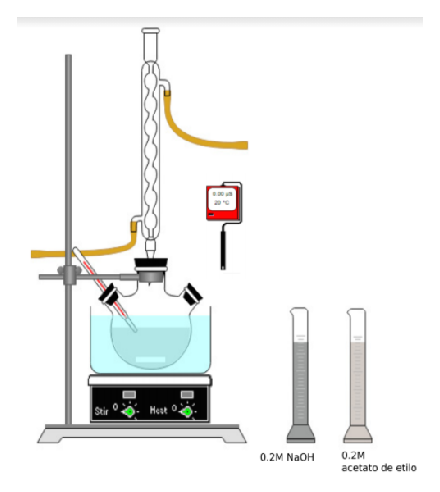
\includegraphics[scale=0.7]{Figuras/Diagrama.eps}
            \caption{Diagrama de la práctica}
        \end{figure}
%
%
%